\chapter{Data Preprocessing}
The dataset consists of retail banking transaction records provided by Novo Banco. Information is distributed across multiple relational tables, including customer identifiers, financial contracts, instruments, and transaction records. Transactions contain information such as booking timestamp, transaction amount, transaction type, and transaction channel .All personal data has been anonymised.

The original data structure is transaction-level, where each row represents a single financial transaction associated with a customer account. Since the objective of this project is to identify suspicious customers rather than suspicious individual transactions, the data were transformed into a customer-level representation.

To capture the overall behaviour of a customer across multiple banking products and accounts, transactions were aggregated at the customer level. A party may be linked to multiple financial contracts and instruments, allowing all activity associated with the same customer to be analysed jointly.

Following aggregation, each row in the modelling dataset corresponds to a single customer, represented by a set of behavioural features derived from the customer's transaction history.
\chapter{Feature Engineering}

This chapter describes the construction of account-level behavioural features used for money mule detection. Since the raw data are recorded at transaction level, features were aggregated at the party level, so that each observation in the modelling dataset corresponds to one customer.

Let \(i\) denote a party and let \(\mathcal{T}_i\) be the set of transactions associated with party \(i\). Each transaction \(j \in \mathcal{T}_i\) has an amount \(x_{ij}\), a booking time \(t_{ij}\), and a direction \(d_{ij} \in \{\mathrm{IN}, \mathrm{OUT}\}\).

\section{Basic Activity Features}

Basic activity features were constructed to describe the overall transaction profile of each party, including transaction frequency, monetary volume, and temporal activity.

The total number of transactions for party \(i\) is defined as
\[
N_i = |\mathcal{T}_i|.
\]
The number of incoming and outgoing transactions are given by
\[
N_i^{in} = \sum_{j \in \mathcal{T}_i} \mathbf{1}(d_{ij}=\mathrm{IN}),
\qquad
N_i^{out} = \sum_{j \in \mathcal{T}_i} \mathbf{1}(d_{ij}=\mathrm{OUT}).
\]
Similarly, the total incoming and outgoing amounts are defined as
\[
A_i^{in} = \sum_{j \in \mathcal{T}_i: d_{ij}=\mathrm{IN}} x_{ij},
\qquad
A_i^{out} = \sum_{j \in \mathcal{T}_i: d_{ij}=\mathrm{OUT}} x_{ij}.
\]

To account for differences in account activity duration, activity-based normalisation was applied. Let \(D_i^{span}\) denote the number of days between the first and last observed transaction for party \(i\), and let \(D_i^{active}\) denote the number of distinct days on which party \(i\) made at least one transaction. Transaction intensity was then measured by
\[
V_i^{span} = \frac{N_i}{\max(D_i^{span},1)},
\qquad
V_i^{active} = \frac{N_i}{\max(D_i^{active},1)}.
\]

Temporal activity features were also included. The off-hours ratio and weekend ratio were defined as
\[
R_i^{off} =
\frac{N_i^{off}}{\max(N_i,1)},
\qquad
R_i^{weekend} =
\frac{N_i^{weekend}}{\max(N_i,1)}.
\]
These features capture whether a customer tends to transact outside standard daytime hours or during weekends.

\section{Amount-Based Transformation Features}

Transaction amounts are typically highly right-skewed, with a small number of very large transactions. To reduce the influence of extreme values, logarithmic transformations were applied to selected amount-based variables:
\[
x^{log} = \log(1+x).
\]
For example, daily incoming and outgoing monetary volumes were transformed as
\[
L_i^{in} =
\log\left(1 + \frac{A_i^{in}}{\max(D_i^{span},1)}\right),
\qquad
L_i^{out} =
\log\left(1 + \frac{A_i^{out}}{\max(D_i^{span},1)}\right).
\]

Additional amount distribution features were constructed to describe the shape of each customer's transaction amount distribution. Let \(m_i\) denote the median transaction amount for party \(i\), \(\bar{x}_i\) the mean transaction amount, \(P_{90,i}\) the 90th percentile, and \(x_{i}^{max}\) the maximum transaction amount. The following features were computed:
\[
G_i = \bar{x}_i - m_i,
\]
\[
G_i^{rel} =
\frac{\bar{x}_i - m_i}{\max(\bar{x}_i,1)},
\]
\[
Q_i^{90/50} =
\frac{P_{90,i}}{\max(m_i,1)},
\qquad
Q_i^{max/50} =
\frac{x_i^{max}}{\max(m_i,1)}.
\]
These features capture whether an account is characterised by occasional unusually large transactions relative to its typical transaction size.

\section{Ratio Features}

Several ratio features were constructed to describe the balance between incoming and outgoing activity. The outgoing transaction ratio and incoming transaction ratio are defined as
\[
R_i^{out,txn} =
\frac{N_i^{out}}{\max(N_i^{in}+N_i^{out},1)},
\qquad
R_i^{in,txn} =
\frac{N_i^{in}}{\max(N_i^{in}+N_i^{out},1)}.
\]
The outgoing amount ratio was defined as
\[
R_i^{out,amt} =
\frac{A_i^{out}}{\max(A_i^{in}+A_i^{out},1)}.
\]
These ratios help distinguish accounts dominated by incoming activity, outgoing activity, or balanced fund movement.

\section{Money Mule Behaviour Features}

Money mule accounts are often characterised by rapid fund forwarding: funds are received and then transferred out shortly afterwards. To capture this behaviour, features were constructed using forward-looking time windows after each incoming transaction. In the final implementation, one-hour and twenty-four-hour windows were retained.

Let \(k\) denote an incoming transaction of party \(i\), with amount \(a_{ik}\) and timestamp \(t_{ik}\). For a time window \(w \in \{1h,24h\}\), define the outgoing amount following this incoming transaction as
\[
O_{ik}^{(w)}
=
\sum_{\substack{j \in \mathcal{T}_i:\\
d_{ij}=\mathrm{OUT},\;
t_{ik}<t_{ij}\leq t_{ik}+w}}
x_{ij}.
\]

\subsection{Near Pass-Through Features}

The pass-through ratio for incoming transaction \(k\) is defined as
\[
P_{ik}^{(w)}
=
\frac{O_{ik}^{(w)}}{\max(a_{ik},1)}.
\]
A near pass-through event is recorded when the outgoing amount is close to the incoming amount:
\[
I_{ik}^{pass,(w)}
=
\mathbf{1}\left(a \leq P_{ik}^{(w)} \leq b\right).
\]
Where a and b are two real number thresholds. The party-level near pass-through ratio is then
\[
R_i^{pass,(w)}
=
\frac{1}{\max(N_i^{in},1)}
\sum_{k=1}^{N_i^{in}}
I_{ik}^{pass,(w)}.
\]
This feature measures the proportion of incoming transactions that are followed by a near-equivalent outflow within the specified time window.

\subsection{One-In-Many-Out Features}

Money mule accounts may also disperse funds through multiple outgoing payments after receiving an incoming transfer. Let
\[
C_{ik}^{out,(w)}
=
\sum_{\substack{j \in \mathcal{T}_i:\\
d_{ij}=\mathrm{OUT},\;
t_{ik}<t_{ij}\leq t_{ik}+w}}
1
\]
be the number of outgoing transactions following incoming transaction \(k\) within window \(w\). A one-in-many-out event is defined as
\[
I_{ik}^{many,(w)}
=
\mathbf{1}\left(C_{ik}^{out,(w)} \geq n\right).
\]
Where n is a threshold. The corresponding party-level ratio is
\[
R_i^{many,(w)}
=
\frac{1}{\max(N_i^{in},1)}
\sum_{k=1}^{N_i^{in}}
I_{ik}^{many,(w)}.
\]
This feature approximates fan-out behaviour, where a single incoming payment is followed by several outgoing payments.

\subsection{Outgoing Intensity and Method Diversity}

In addition to the ratio features, the maximum number of outgoing transactions following any incoming transaction was recorded:
\[
M_i^{out,(w)}
=
\max_k C_{ik}^{out,(w)}.
\]
This captures the most intense observed fund dispersion event for each party.

For the one-hour window, outgoing method diversity was also computed as the number of distinct outgoing transaction types following an incoming transaction:
\[
D_{ik}^{method,(1h)}
=
\left|
\left\{
\mathrm{type}_{ij}:
d_{ij}=\mathrm{OUT},
\;
t_{ik}<t_{ij}\leq t_{ik}+1h
\right\}
\right|.
\]
The maximum method diversity across incoming anchors was then used as a party-level feature:
\[
D_i^{method}
=
\max_k D_{ik}^{method,(1h)}.
\]

Counterparty information was not included in the current implementation due to computational constraints. Therefore, fan-out behaviour is approximated using the number of outgoing transactions rather than the number of distinct beneficiaries.
\subsection{Drain Ratio}

The near pass-through features described above are count-based: they measure the proportion of incoming transactions that are followed by approximately equivalent outgoing transfers. However, this may lose information about monetary importance. For example, several small incoming transactions may dominate the count-based ratio, while a single large incoming transfer that is rapidly drained may have greater relevance from a money mule detection perspective.

To incorporate the monetary scale of the behaviour, a drain ratio feature was constructed. For each incoming transaction \(k\) of party \(i\), with amount \(a_{ik}\), outgoing transactions occurring within a predefined window \(w\) (1h/24h) after the incoming transaction are considered. Outgoing amounts are allocated using a First-In-First-Out (FIFO) matching procedure, so that each outgoing amount is assigned to the earliest eligible incoming transaction and cannot be counted multiple times.

Let \(D_{ik}^{(w)}\) denote the amount of incoming transaction \(k\) that is drained through outgoing transfers within window \(w\). The party-level drain ratio is then defined as
\[
R_i^{\mathrm{drain},(w)}
=
\frac{\sum_{k=1}^{N_i^{in}} D_{ik}^{(w)}}
{\sum_{k=1}^{N_i^{in}} a_{ik}}.
\]

This feature measures the proportion of the total inbound monetary volume over the customer's observed transaction history that is transferred out within a short period of receipt. Unlike the near pass-through ratio, it is amount-weighted and does not require the outgoing amount to be close to the incoming amount for each individual transaction.

\begin{figure}[ht]
    \centering
    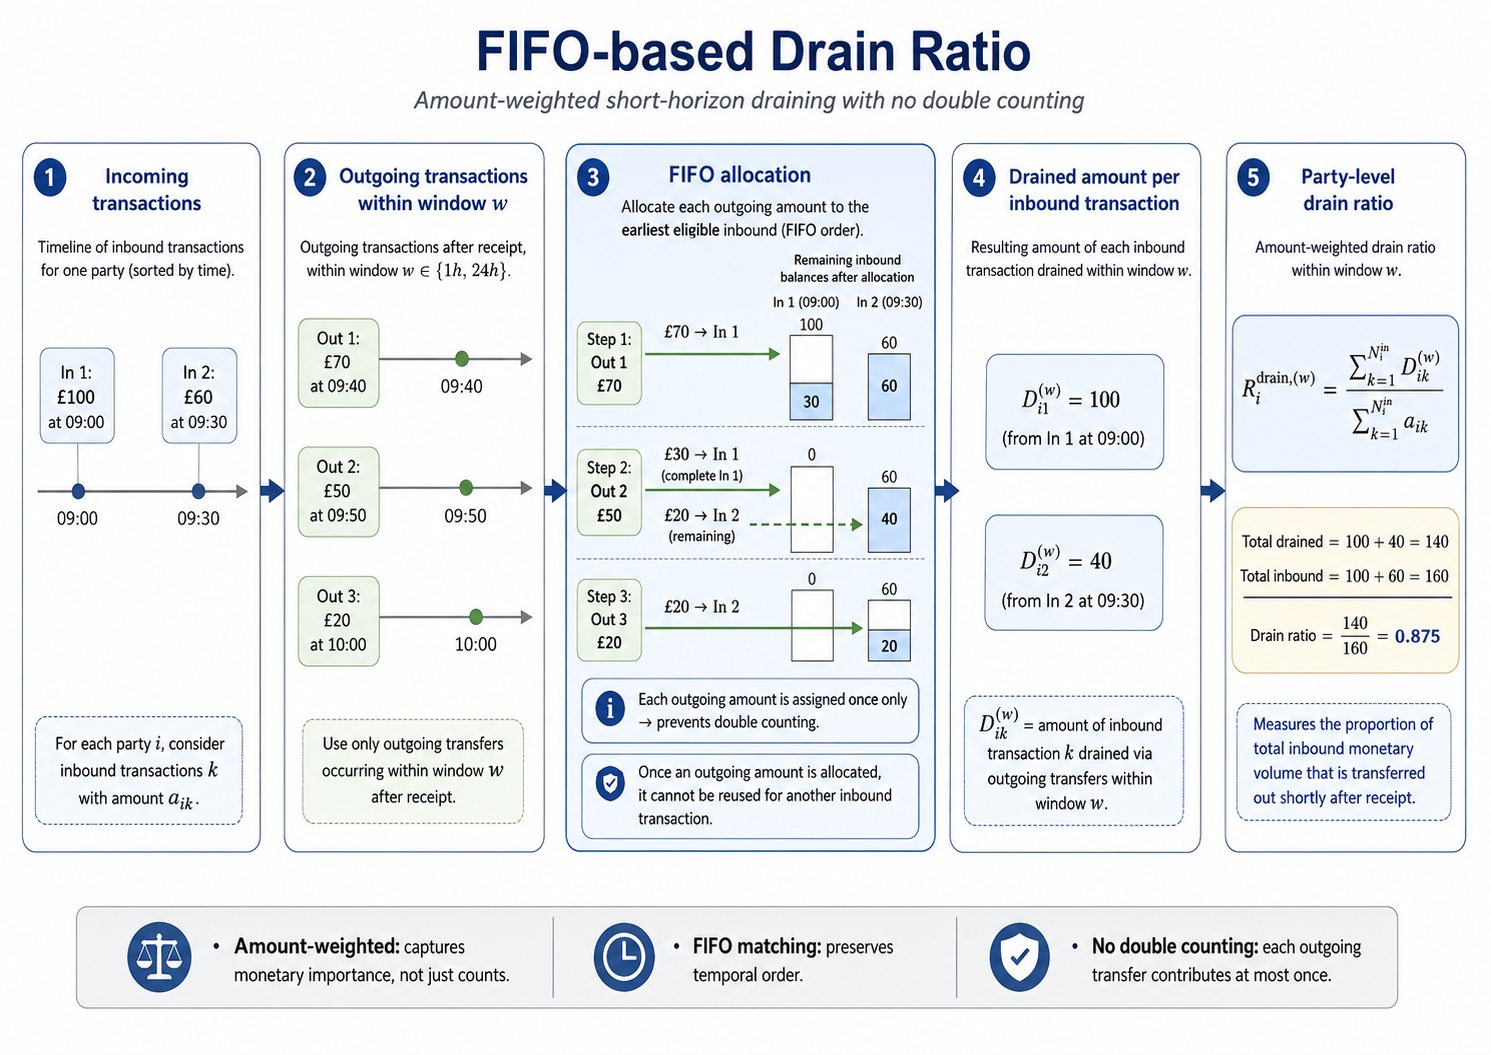
\includegraphics[width=0.55\textwidth]{methods/ChatGPT Image 2026年6月20日 13_20_06.png}
    \caption{FIFO drain diagram}
    \label{fig:autoencoder_architecture}
\end{figure}
\chapter{Methods}
\section{DBSCAN}
Density-Based Spatial Clustering of Applications with Noise (DBSCAN) was used as the main unsupervised clustering method \cite{ester1996density}. DBSCAN is suitable for this problem because it does not require the number of clusters to be specified in advance and explicitly identifies observations that do not belong to any dense region as noise. This is useful in the context of money mule detection, where suspicious accounts are expected to form a small minority of the population and may not constitute a well-separated spherical cluster.  
\begin{figure} 
    \centering
    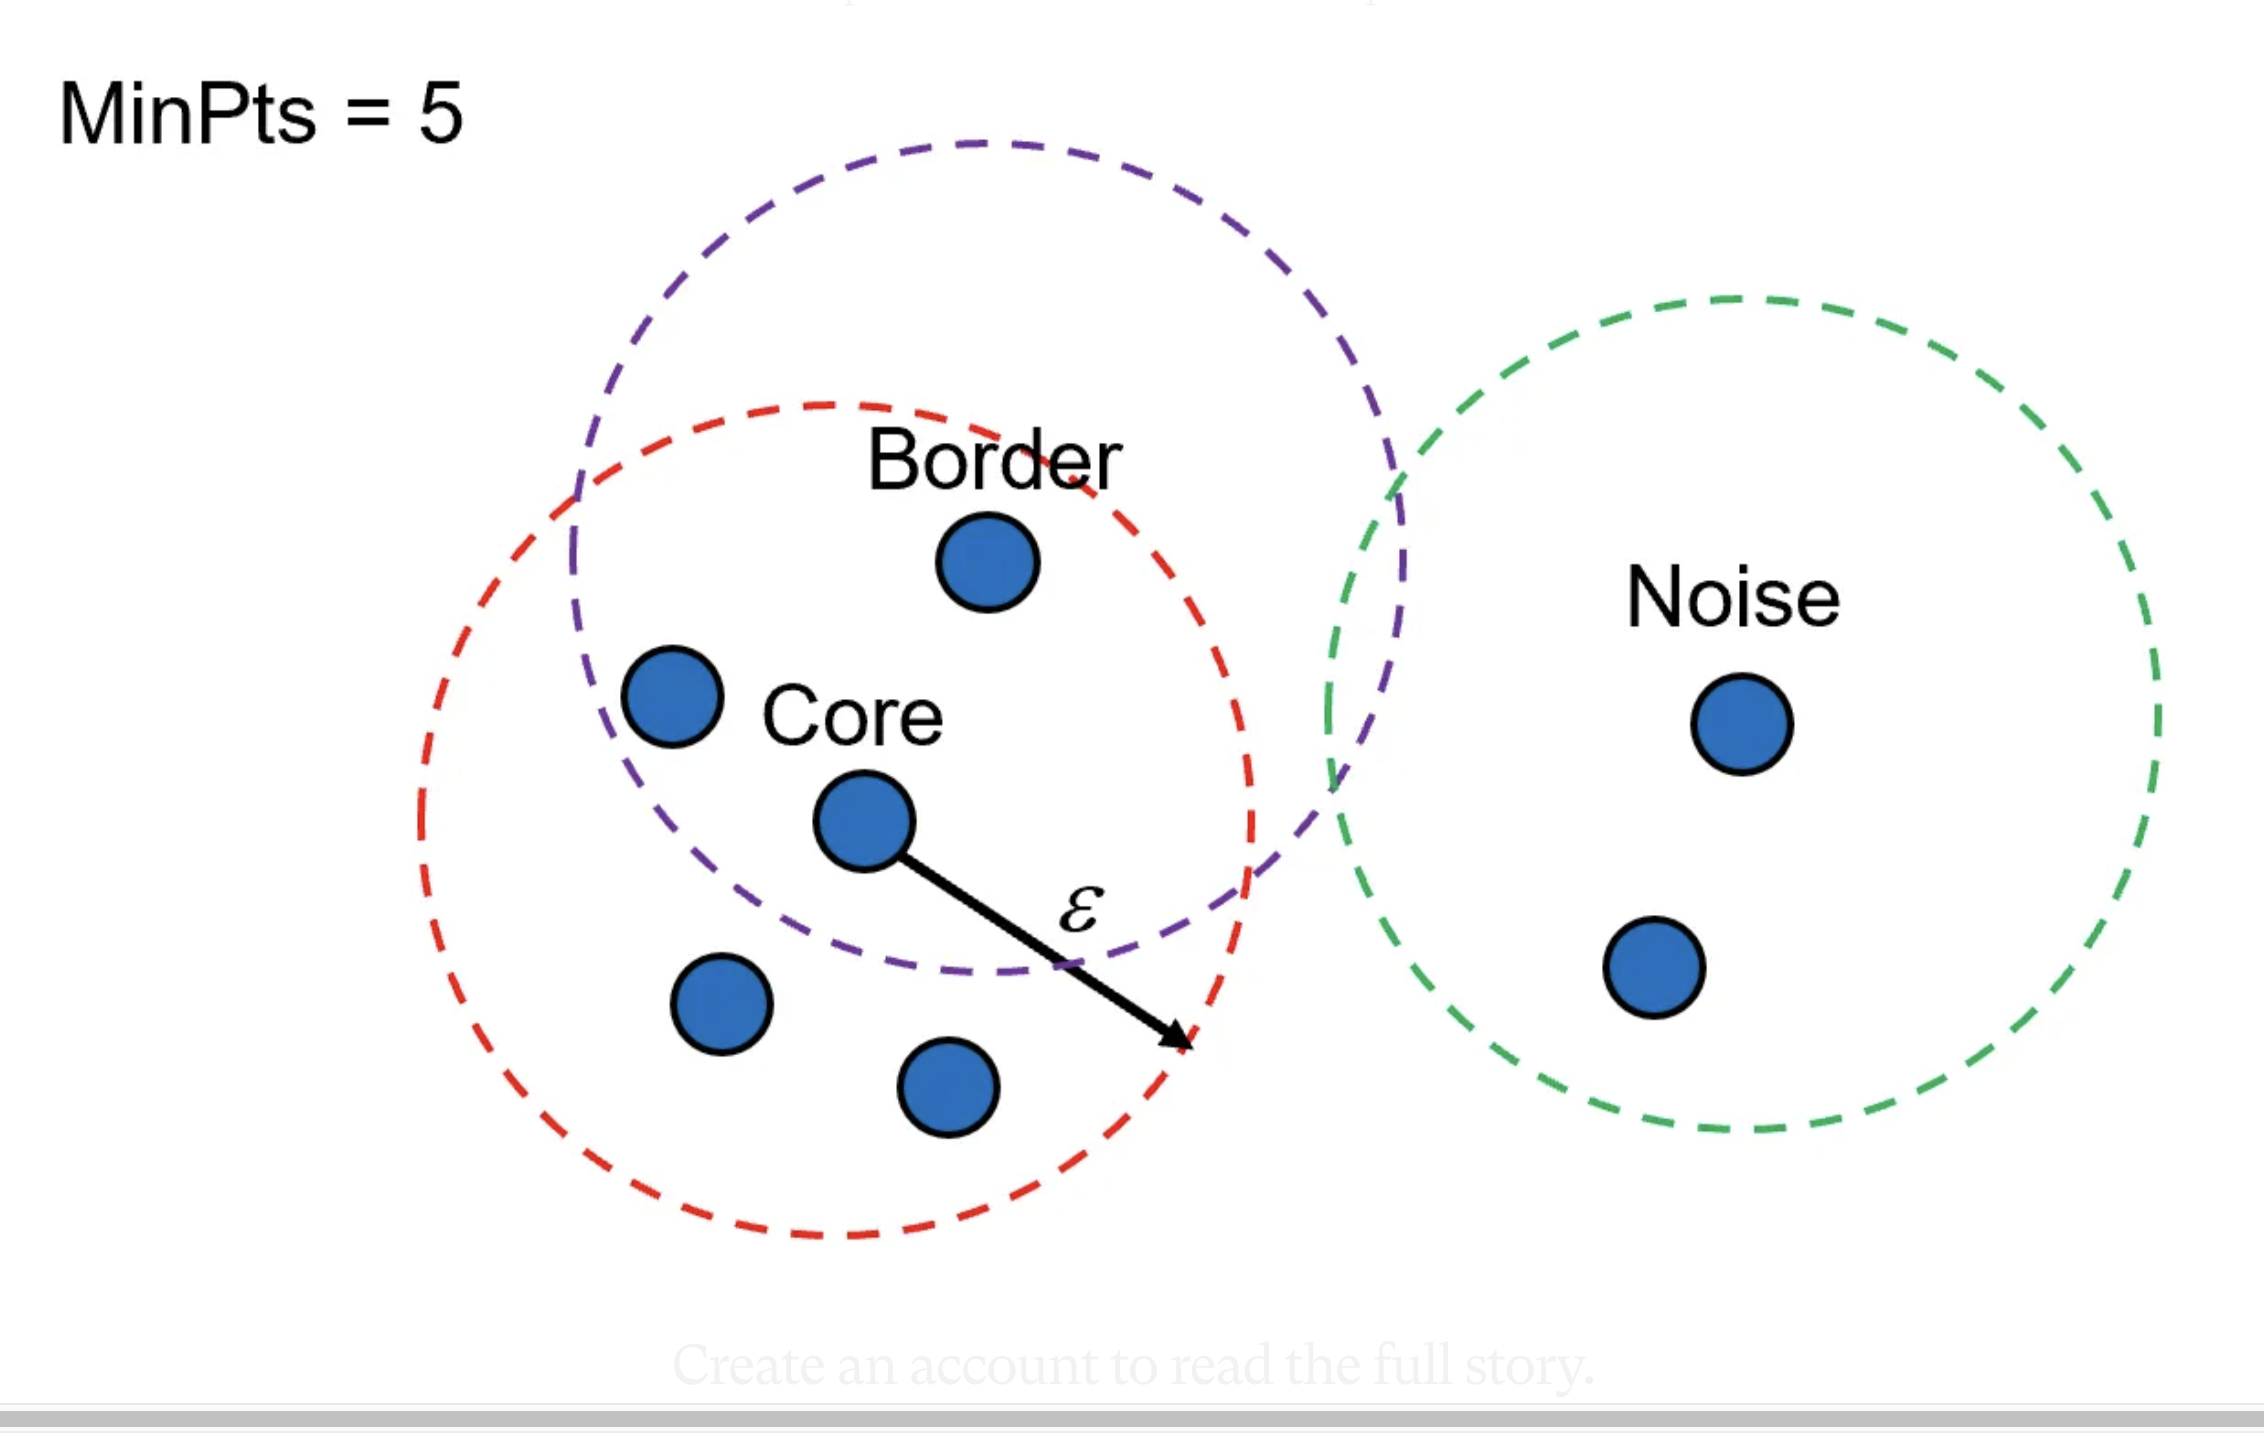
\includegraphics[width=0.55\textwidth]{methods/Screenshot 2026-06-18 at 19.35.24.png} 
    \caption{DBSCAN with MinPts=5}
    \label{fig:autoencoder_architecture}
\end{figure}
Let
\[
X = \{x_1,\ldots,x_n\} \subset \mathbb{R}^p
\]
denote the set of customer-level feature vectors, where each \(x_i\) represents one party. Prior to clustering, all numerical features were standardised to have zero mean and unit variance, since DBSCAN relies on distances between observations.

DBSCAN is controlled by two parameters: the neighbourhood radius \(\varepsilon > 0\) and the minimum number of neighbouring points required to form a dense region, denoted by \(\text{MinPts}\). For a point \(x_i\), its \(\varepsilon\)-neighbourhood is defined as
\[
N_{\varepsilon}(x_i)
=
\left\{
x_j \in X :
d(x_i,x_j) \leq \varepsilon
\right\},
\]
where \(d(\cdot,\cdot)\) is the distance metric. In this project, Euclidean distance was used:
\[
d(x_i,x_j)
=
\left(
\sum_{l=1}^{p}
(x_{il}-x_{jl})^2
\right)^{1/2}.
\]


A point \(x_i\) is defined as a core point if
\[
|N_{\varepsilon}(x_i)| \geq \text{MinPts}.
\]
A point \(x_j\) is directly density-reachable from \(x_i\) if \(x_j \in N_{\varepsilon}(x_i)\) and \(x_i\) is a core point. More generally, \(x_j\) is density-reachable from \(x_i\) if there exists a sequence of points
\[
x_i = z_0, z_1, \ldots, z_m = x_j
\]
such that each \(z_{r+1}\) is directly density-reachable from \(z_r\). A cluster is then defined as a maximal set of density-connected points. Points that are not density-reachable from any core point are labelled as noise.

This distinction is important for money mule detection. The largest dense region is expected to represent common retail behaviour, while noise points and small dense regions may correspond to unusual customer behaviour. Therefore, DBSCAN was used not as a definitive classifier, but as a first-stage segmentation method to reduce the search space and identify accounts requiring further profiling.
\begin{figure} [H]
    \centering
    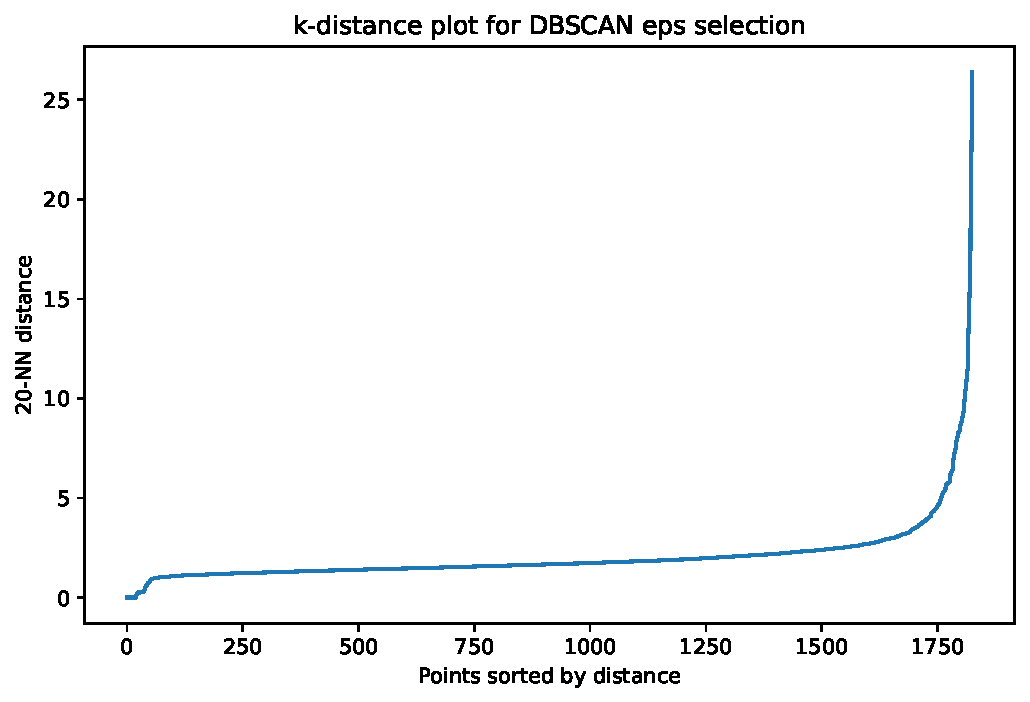
\includegraphics[width=0.55\textwidth]{k_distance_plot.pdf} 
    \caption{k Distance Plot} 
    \label{fig:autoencoder_architecture}
\end{figure}
To guide the choice of \(\varepsilon\), the sorted \(k\)-distance graph heuristic was used, 
as suggested by \cite{ester1996density}. Let $d_k(x_i)$ denote the distance from observation $x_i$ to its $k$-th nearest neighbour, where $k=\text{MinPts}$. Since $\text{MinPts}=20$ in the final implementation, $d_{20}(x_i)$ was computed for every observation. The resulting distances were sorted in ascending order,

\[
d_{(1)} \le d_{(2)} \le \cdots \le d_{(n)},
\]
and plotted against their rank $i$. The horizontal axis therefore represents the ordered index of the observations after sorting, while the vertical axis represents the corresponding $20$-nearest-neighbour distance.

The quantity $d_k(x_i)$ provides a local measure of density around $x_i$. Small values of $d_k(x_i)$ indicate that at least $k$ neighbouring observations lie within a relatively small radius, corresponding to a dense region of the feature space. Conversely, large values indicate that a substantially larger radius is required to encompass $k$ neighbours, suggesting a lower local density.

Equivalently, the DBSCAN core-point condition

\[
|N_{\varepsilon}(x_i)| \ge \text{MinPts}
\]

implies that the distance from $x_i$ to its $k$-th nearest neighbour must satisfy

\[
d_k(x_i) \le \varepsilon.
\]

Consequently, the sorted $k$-distance curve provides information about the distribution of local densities in the dataset. The relatively flat section of the curve corresponds to observations located in dense regions, whereas the rapidly increasing section corresponds to observations in progressively sparser regions. The transition between these two regimes appears as an elbow in the curve.

The parameter $\varepsilon$ was selected near this elbow point. Choosing a substantially smaller value would classify many observations from dense regions as noise, whereas choosing a substantially larger value would merge sparse regions with the main cluster and reduce the ability of DBSCAN to identify anomalous observations. Therefore, the elbow point can be interpreted as an empirical estimate of the density threshold separating the dominant high-density population from lower-density observations. For the present dataset, the elbow occurred at approximately $\varepsilon \approx 4.5/ 5$, which was adopted in the final model.

Sensitivity checks were subsequently performed by comparing the number of clusters and the proportion of noise observations under nearby values of $\varepsilon$.

In the final DBSCAN implementation, \(\text{MinPts}=20\) was used. The selected value of \(\varepsilon\) produced one large cluster representing the majority of retail customers and a smaller set of noise observations. The noise observations were subsequently ranked using mule-behaviour features such as near pass-through ratios, one-in-many-out ratios, and forwarding intensity features.

\section{Autoencoder}

Let
\[
X=\{x_i\}_{i=1}^{n}, \qquad x_i\in\mathbb{R}^{d},
\]
denote the set of account-level feature vectors after preprocessing and
standardisation, where \(d=17\) is the number of input features. Equivalently,
the data matrix may be written as \(X\in\mathbb{R}^{n\times d}\), where each row
corresponds to one account.
\begin{figure}[htbp]
    \centering
    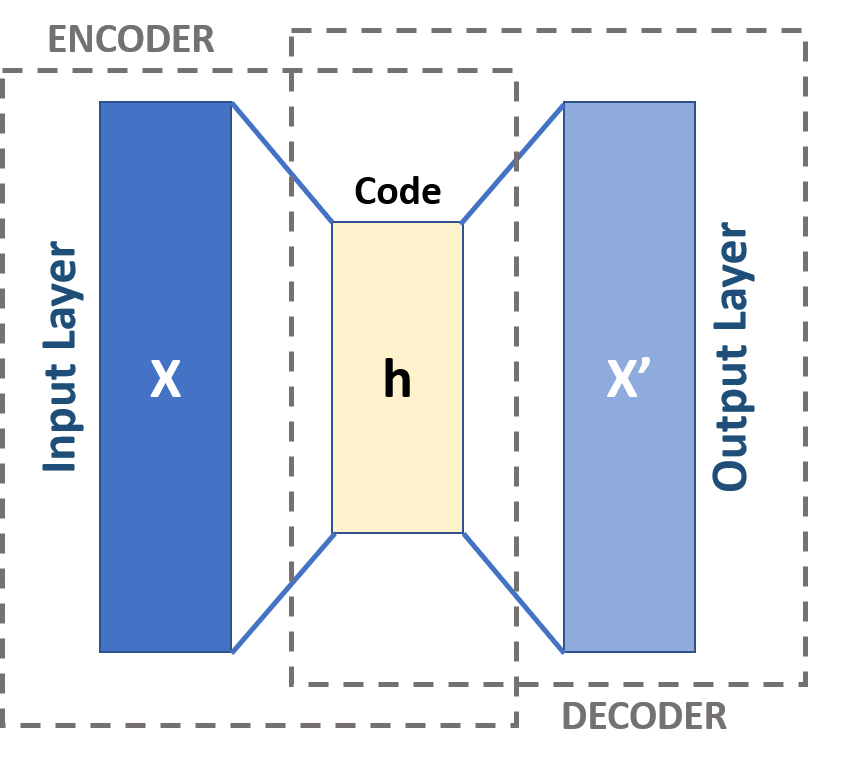
\includegraphics[width=0.55\textwidth]{methods/Autoencoder_schema.png}
    \caption{Schematic representation of an autoencoder architecture.}
    \label{fig:autoencoder_architecture}
\end{figure}
An autoencoder was used as an unsupervised reconstruction model. The objective
of the model is to learn a lower-dimensional representation of each input vector
and then reconstruct the original feature vector from this representation. Let
\[
E_{\phi}:\mathbb{R}^{d}\rightarrow\mathbb{R}^{q}
\]
denote the encoder, where \(\phi\) represents the encoder parameters and
\(q<d\) is the dimension of the latent space. For each observation \(x_i\), the
encoder produces a latent representation
\[
z_i=E_{\phi}(x_i), \qquad z_i\in\mathbb{R}^{q}.
\]
Let
\[
D_{\theta}:\mathbb{R}^{q}\rightarrow\mathbb{R}^{d}
\]
denote the decoder, where \(\theta\) represents the decoder parameters. The
decoder maps the latent representation back to the original feature space:
\[
\hat{x}_i=D_{\theta}(z_i).
\]
Therefore, the full autoencoder mapping is given by
\[
\hat{x}_i=D_{\theta}(E_{\phi}(x_i)).
\]

In this study, the autoencoder was implemented as a fully connected multilayer
perceptron with architecture
\[
17 \rightarrow 8 \rightarrow 4 \rightarrow 8 \rightarrow 17.
\]
The middle layer of dimension \(q=4\) acts as the bottleneck representation. The
hidden layers use the ReLU activation function
\[
\sigma(u)=\max(0,u),
\]
while the output layer is linear, since the task is to reconstruct continuous
standardised features.

More explicitly, the encoder is given by
\[
a_i^{(1)}
=
\sigma\left(W_E^{(1)}x_i+b_E^{(1)}\right),
\]
\[
z_i
=
E_{\phi}(x_i)
=
\sigma\left(W_E^{(2)}a_i^{(1)}+b_E^{(2)}\right),
\]
where
\[
\phi
=
\left\{
W_E^{(1)},b_E^{(1)},W_E^{(2)},b_E^{(2)}
\right\}
\]
denotes the collection of encoder parameters. The decoder is given by
\[
a_i^{(3)}
=
\sigma\left(W_D^{(1)}z_i+b_D^{(1)}\right),
\]
\[
\hat{x}_i
=
D_{\theta}(z_i)
=
W_D^{(2)}a_i^{(3)}+b_D^{(2)},
\]
where
\[
\theta
=
\left\{
W_D^{(1)},b_D^{(1)},W_D^{(2)},b_D^{(2)}
\right\}
\]
denotes the collection of decoder parameters.

The autoencoder is trained by minimising the discrepancy between each input
vector and its reconstruction. In general, the autoencoder objective can be
written as
\[
L(\theta,\phi)
:=
\mathbb{E}_{x\sim\mu_{\mathrm{ref}}}
\left[
d\left(x,D_{\theta}(E_{\phi}(x))\right)
\right],
\]
where \(\mu_{\mathrm{ref}}\) denotes the reference distribution of the training
data and \(d(\cdot,\cdot)\) is a reconstruction distance.

In this implementation, the squared Euclidean distance was used:
\[
d(x,\hat{x})
=
\|x-\hat{x}\|_2^2.
\]
Hence, for the finite training sample \(X=\{x_i\}_{i=1}^{n}\), the empirical
reconstruction loss becomes
\[
\widehat{L}(\theta,\phi)
=
\frac{1}{n}
\sum_{i=1}^{n}
\left\|
x_i-D_{\theta}(E_{\phi}(x_i))
\right\|_2^2.
\]
Equivalently,
\[
\widehat{L}(\theta,\phi)
=
\frac{1}{n}
\sum_{i=1}^{n}
\sum_{j=1}^{d}
\left(x_{ij}-\hat{x}_{ij}\right)^2,
\]
where
\[
\hat{x}_i=D_{\theta}(E_{\phi}(x_i)).
\]
The model was trained using the Adam optimiser with backpropagation. Let
\[
\Theta=(\theta,\phi)
\]
denote the collection of all trainable parameters in the encoder and decoder.
At iteration \(t\), Adam computes a stochastic gradient of the empirical
reconstruction loss over a minibatch \(B_t\):
\[
g_t
=
\nabla_{\Theta}
\left[
\frac{1}{|B_t|}
\sum_{x_i\in B_t}
\left\|
x_i-D_{\theta}(E_{\phi}(x_i))
\right\|_2^2
\right].
\]
Adam maintains exponentially weighted estimates of the first and second moments
of the gradient:
\[
m_t
=
\beta_1 m_{t-1} + (1-\beta_1)g_t,
\]
\[
v_t
=
\beta_2 v_{t-1} + (1-\beta_2)(g_t\odot g_t),
\]
where \(\odot\) denotes element-wise multiplication. The bias-corrected moment
estimates are
\[
\hat{m}_t
=
\frac{m_t}{1-\beta_1^t},
\qquad
\hat{v}_t
=
\frac{v_t}{1-\beta_2^t}.
\]
The parameters are then updated according to
\[
\Theta_t
=
\Theta_{t-1}
-
\eta
\frac{\hat{m}_t}{\sqrt{\hat{v}_t}+\epsilon},
\]
where \(\eta\) is the learning rate and \(\epsilon\) is a small constant used for
numerical stability. In this implementation, the Adam optimiser was used with
learning rate \(\eta=10^{-3}\), \(\beta_1=0.9\), \(\beta_2=0.999\), and
\(\epsilon=10^{-8}\).
```
After training, each account is assigned a reconstruction error score:
\[
s_i
=
\left\|x_i-\hat{x}_i\right\|_2^2
=
\sum_{j=1}^{d}
\left(x_{ij}-\hat{x}_{ij}\right)^2.
\]
Accounts with larger reconstruction errors are interpreted as less well
represented by the patterns learned by the autoencoder. In the context of
anomaly detection, a high reconstruction error suggests that the account's
behaviour differs from the dominant patterns in the training data, and such
accounts are therefore treated as more suspicious candidates for further
investigation.

The underlying assumption is that the majority of accounts in the training data
represent normal behaviour. The autoencoder learns to reconstruct these common
behavioural patterns well, while unusual accounts, such as potential money mule
accounts, are expected to produce larger reconstruction errors.
\section{Supervised Learning}
After the unsupervised experiments, a small set of confirmed mule accounts became available from Novobanco. This allowed an additional supervised modelling experiment to be conducted. The confirmed mule parties were appended to the previously constructed retail party sample, and a binary indicator was created, where confirmed mule parties were assigned label 1 and all remaining sampled retail parties were treated as unlabelled controls with label 0.
Two supervised models were fitted: a class-weighted logistic regression model and a class-weighted XGBoost classifier. Class weighting was used because confirmed mule accounts represented only a small minority of the modelling dataset. This increases the penalty for misclassifying confirmed mule accounts and reduces the tendency of the model to predict the majority unlabelled class for all observations.
\subsection{Logistic Regression}
Logistic regression was used as a supervised linear baseline for binary mule classification. 
It models the conditional probability of the positive class through a logistic transformation 
of a linear predictor, making the log-odds a linear function of the input features 
\citep{cox1958regression}.
Let
\[
x_i \in \mathbb{R}^{p},
\qquad
y_i \in \{0,1\},
\qquad
i=1,\ldots,N,
\]

denote the feature vector and binary label for party \(i\), where \(p\) is the number
of selected behavioural features.

Logistic regression assumes that the log-odds of the positive class is a linear
function of the input variables:

\[
\log
\left(
\frac{\Pr(y_i=1 \mid x_i)}
{\Pr(y_i=0 \mid x_i)}
\right)
=
\beta_0 + x_i^{T}\beta,
\]

where \(\beta_0\) is the intercept and
\(\beta \in \mathbb{R}^{p}\) is the coefficient vector.

Rearranging the above expression yields

\[
p_i
=
\Pr(y_i=1 \mid x_i)
=
\frac{1}
{1+\exp\left[-(\beta_0+x_i^{T}\beta)\right]}.
\]

Under this formulation, the response variable is assumed to follow a Bernoulli
distribution,

\[
y_i \sim \mathrm{Bernoulli}(p_i).
\]

Assuming independent observations, the likelihood function is

\[
L(\beta)
=
\prod_{i=1}^{N}
p_i^{y_i}
(1-p_i)^{1-y_i}.
\]

Taking logarithms gives the log-likelihood

\[
\ell(\beta)
=
\sum_{i=1}^{N}
\left[
y_i \log(p_i)
+
(1-y_i)\log(1-p_i)
\right].
\]

The model parameters were estimated by minimising the negative log-likelihood.
Since confirmed mule accounts represented only a small minority of the modelling
dataset, a class-weighted version of the loss function was used\citep{he2009learning}:

\[
L(\beta)
=
-\sum_{i=1}^{N}
w_{y_i}
\left[
y_i \log(p_i) + (1-y_i)\log(1-p_i)
\right]
+
\lambda \|\beta\|_2^2,
\]

where \(\lambda \|\beta\|_2^2\) denotes the \(L_2\) regularisation penalty, which shrinks large coefficients and helps stabilise the model when behavioural features are correlated.  \(w_{y_i}\) denotes the class weight assigned to observation \(i\).
For the scikit-learn implementation \cite{sklearn_logistic} with \texttt{class\_weight="balanced"}, the class weight for class \(c\) is defined as
\[
w_c = \frac{N}{K N_c} ,
\]
where \(N\) is the number of training observations, \(K\) is the number of classes, and \(N_c\) is the number of observations belonging to class \(c\) in the training set. In this experiment, the training set contained 1506 unlabeled observations and 72 confirmed mule observations. Therefore, the corresponding class weights were
\[
w_0 = \frac{1578}{2 \times 1506} \approx 0.524,
\qquad
w_1 = \frac{1578}{2 \times 72} \approx 10.958.
\]

Thus, errors on confirmed mule observations received substantially larger weight than errors on unlabeled observations. This was intended to reduce the tendency of the model to favour the majority unlabeled class and to improve sensitivity to the minority confirmed mule class.


The model was implemented using the \texttt{LogisticRegression} estimator from
the \texttt{scikit-learn} package with \texttt{class\_weight="balanced"}.
The optimisation of the coefficient vector was performed automatically by the
underlying numerical optimisation algorithm.
\subsection{XGBoost}
As a second supervised baseline, an XGBoost classifier was used. XGBoost, introduced by \cite{Chen_2016}, is a scalable gradient tree boosting method that constructs an additive ensemble of decision trees. While logistic
regression models the log-odds as a linear function of the input features, XGBoost
constructs a non-linear additive model of decision trees. This makes it suitable for
capturing interaction effects between behavioural features, such as high draining
activity combined with one-in-many-out transfer patterns.

Let \(x_i \in \mathbb{R}^{p}\) denote the feature vector for party \(i\), and let
\(y_i \in \{0,1\}\) denote the binary label. XGBoost models the prediction as an
additive ensemble of regression trees,

\[
\hat{z}_i
=
\sum_{k=1}^{K} f_k(x_i),
\qquad
f_k \in \mathcal{F},
\]

where \(\mathcal{F}\) denotes the space of regression trees and \(\hat{z}_i\) is the
raw prediction score before applying the logistic transformation. For binary
classification, the predicted probability of the positive class is obtained by

\[
\hat{p}_i
=
\sigma(\hat{z}_i)
=
\frac{1}{1+\exp(-\hat{z}_i)}.
\]

The objective function consists of a training loss and a regularisation penalty on
the complexity of the trees:

\[
\mathcal{L}
=
\sum_{i=1}^{N}
l(y_i,\hat{p}_i)
+
\sum_{k=1}^{K}
\Omega(f_k),
\]

where \(l(y_i,\hat{p}_i)\) is the binary logistic loss,

\[
l(y_i,\hat{p}_i)
=
-
\left[
y_i\log(\hat{p}_i)
+
(1-y_i)\log(1-\hat{p}_i)
\right].
\]

The regularisation term penalises overly complex trees and is commonly written as

\[
\Omega(f)
=
\gamma T
+
\frac{1}{2}\lambda
\sum_{j=1}^{T}
w_j^2,
\]

where \(T\) is the number of leaves in the tree, \(w_j\) is the score assigned to
leaf \(j\), and \(\gamma\) and \(\lambda\) are regularisation parameters.

XGBoost fits trees sequentially. Suppose that after \(t-1\) boosting iterations the
current raw prediction for observation \(i\) is \(\hat{z}_i^{(t-1)}\). At iteration
\(t\), a new tree \(f_t\) is added, giving

\[
\hat{z}_i^{(t)}
=
\hat{z}_i^{(t-1)}
+
f_t(x_i).
\]

The objective at iteration \(t\) is therefore

\[
\mathcal{L}^{(t)}
=
\sum_{i=1}^{N}
l\left(y_i,\sigma\left(\hat{z}_i^{(t-1)}+f_t(x_i)\right)\right)
+
\Omega(f_t).
\]

Rather than optimising this objective directly, XGBoost uses a second-order Taylor
approximation of the loss around the current predictions:

\[
\mathcal{L}^{(t)}
\approx
\sum_{i=1}^{N}
\left[
g_i f_t(x_i)
+
\frac{1}{2}h_i f_t(x_i)^2
\right]
+
\Omega(f_t),
\]

where

\[
g_i
=
\frac{\partial l(y_i,\hat{p}_i)}
{\partial \hat{z}_i},
\qquad
h_i
=
\frac{\partial^2 l(y_i,\hat{p}_i)}
{\partial \hat{z}_i^2}.
\]

For logistic loss, these terms are

\[
g_i = \hat{p}_i - y_i,
\qquad
h_i = \hat{p}_i(1-\hat{p}_i).
\]

Each tree partitions the observations into leaves. Let \(I_j\) denote the set of
observations assigned to leaf \(j\). The sum of first-order and second-order
gradient statistics in leaf \(j\) are

\[
G_j = \sum_{i \in I_j} g_i,
\qquad
H_j = \sum_{i \in I_j} h_i.
\]

For a fixed tree structure, the optimal leaf weight is

\[
w_j^{*}
=
-
\frac{G_j}{H_j+\lambda}.
\]

Substituting this back into the objective gives the approximate optimal value of a
tree:

\[
\tilde{\mathcal{L}}^{(t)}
=
-
\frac{1}{2}
\sum_{j=1}^{T}
\frac{G_j^2}{H_j+\lambda}
+
\gamma T.
\]

This expression shows how XGBoost chooses splits. For a candidate split dividing a
node into left and right child nodes, the split gain is

\[
\mathrm{Gain}
=
\frac{1}{2}
\left[
\frac{G_L^2}{H_L+\lambda}
+
\frac{G_R^2}{H_R+\lambda}
-
\frac{(G_L+G_R)^2}{H_L+H_R+\lambda}
\right]
-
\gamma.
\]

A split is selected when it provides a positive improvement in the regularised
objective. This mechanism allows XGBoost to build trees greedily while controlling
overfitting through the regularisation parameters.

Since confirmed mule accounts formed only a small minority of the modelling dataset, class
imbalance was handled using the parameter \texttt{scale\_pos\_weight}. This parameter increases the
contribution of positive observations in the training objective. In the implementation \cite{xgboost_parameters} , it was set
as
\[
\texttt{scale\_pos\_weight} = \frac{N_0}{N_1},
\]
where \(N_0\) is the number of unlabeled observations and \(N_1\) is the number of confirmed mule
observations in the training set. In this experiment, the training set contained 1506 unlabeled
observations and 72 confirmed mule observations. Therefore,
\[
\texttt{scale\_pos\_weight}
=
\frac{1506}{72}
\approx 20.92.
\]
This gives greater weight to confirmed mule observations during training and reduces the
tendency of the model to favour the majority unlabeled class.
The model was implemented using the \texttt{XGBClassifier} estimator. As with the
logistic regression model, the output scores were interpreted as relative mule-risk
scores rather than calibrated probabilities, since the confirmed mule accounts were
appended to a random retail sample.

To interpret the XGBoost model, SHAP values were computed as a post-hoc explanation method. SHAP is based on Shapley values from cooperative game theory and decomposes each model prediction into additive feature contributions \citep{lundberg2017unified}. For an observation \(i\), the model output can be written as
\[
f(x_i) = \mathbb{E}[f(X)] + \sum_{j=1}^{p} \phi_{ij},
\]
where \(\mathbb{E}[f(X)]\) is the baseline model output and \(\phi_{ij}\) is the SHAP value of feature \(j\) for observation \(i\). A positive SHAP value indicates that the feature pushes the prediction towards the confirmed mule class, while a negative SHAP value pushes the prediction towards the unlabeled comparison class. Global feature importance was measured using the mean absolute SHAP value,
\[
I_j = \frac{1}{N}\sum_{i=1}^{N} |\phi_{ij}|.
\]
The SHAP summary plot was used to visualise both the magnitude and direction of feature effects for the XGBoost classifier.